\subsection{Ca sử dụng xem danh sách địa điểm gần người dùng}
\noindent Ca sử dụng này mô tả cách người dùng tìm kiếm và xem danh sách các địa điểm (du lịch, nhà hàng, khách sạn) ở gần vị trí hiện tại của họ. Hệ thống yêu cầu quyền truy cập vị trí để thực hiện chức năng này. Bảng~\ref{tab:uc_nearby_places_spec} trình bày chi tiết đặc tả ca sử dụng, bao gồm luồng sự kiện chính, luồng thay thế, các điều kiện và yêu cầu liên quan. Các biểu đồ hoạt động, quan hệ (Bảng~\ref{tab:uc_nearby_places_diagrams}) và tuần tự (Hình~\ref{fig:3-3-7-sequence-diagram}) minh họa rõ hơn về quy trình và tương tác hệ thống.
% \vspace{0.5cm} % Adjust spacing if needed

% Use longtable environment
% Need \usepackage{longtable} and \usepackage{calc} in preamble
\begin{longtable}{| p{4cm} | p{\dimexpr\linewidth-4cm-4\tabcolsep} |} % Adjust widths as needed
    \caption{Đặc tả ca sử dụng xem danh sách địa điểm gần người dùng.} % Caption inside longtable
    \label{tab:uc_nearby_places_spec} \\ % Label after caption

    \hline
    \textbf{Mô tả} & Người dùng xem danh sách địa điểm du lịch, nhà hàng, khách sạn gần bản thân. \\
    \hline
    \endfirsthead % Header for the first page

    % No \endhead content needed

    % No \endfoot content needed

    \hline % Footer for the last page
    \endlastfoot

    % --- Table Content ---
    \textbf{Luồng cơ bản} & 1. Người dùng truy cập tab khám phá và bấm vào thanh tìm kiếm. \newline
                           2. Người dùng bấm vào biểu tượng "Lân cận". \newline
                           3. Hệ thống hiển thị hộp thoại cấp quyền thông tin vị trí hiện tại. \newline
                           4. Người dùng cấp quyền cho hệ thống. \newline
                           5. Hệ thống lấy vị trí hiện tại của người dùng và hiển thị danh sách địa điểm gần nhất. \\
    \hline
    \textbf{Luồng thay thế} & Người dùng không cấp quyền truy cập vị trí sẽ nhận thông báo lỗi. \\
    \hline
    \textbf{Tiền điều kiện} & Người dùng đang đăng nhập và phiên đăng nhập chưa kết thúc. \\
    \hline
    \textbf{Hậu điều kiện} & - Người dùng có thể xem địa chỉ của bản thân và xem chi tiết các dịch vụ, địa điểm trong danh sách. \newline
                           - Người dùng có thể xem dạng bản đồ các địa điểm trong danh sách. \\
    \hline
    \textbf{Yêu cầu phi chức năng} & Hệ thống xử lý lấy danh sách không quá 5s. \\
    % --- End Table Content ---

\end{longtable}
\vspace{0.8cm}

\begin{table}[H] % Wrap the diagrams table
    \centering
    \caption{Biểu đồ hoạt động ca sử dụng xem danh sách địa điểm gần người dùng.} % Add caption
    \label{tab:uc_nearby_places_diagrams} % Add label
    \begin{tabular}{| c | c |}
        \hline
        \textbf{Biểu đồ hoạt động} & \textbf{Quan hệ} \\
        \hline
        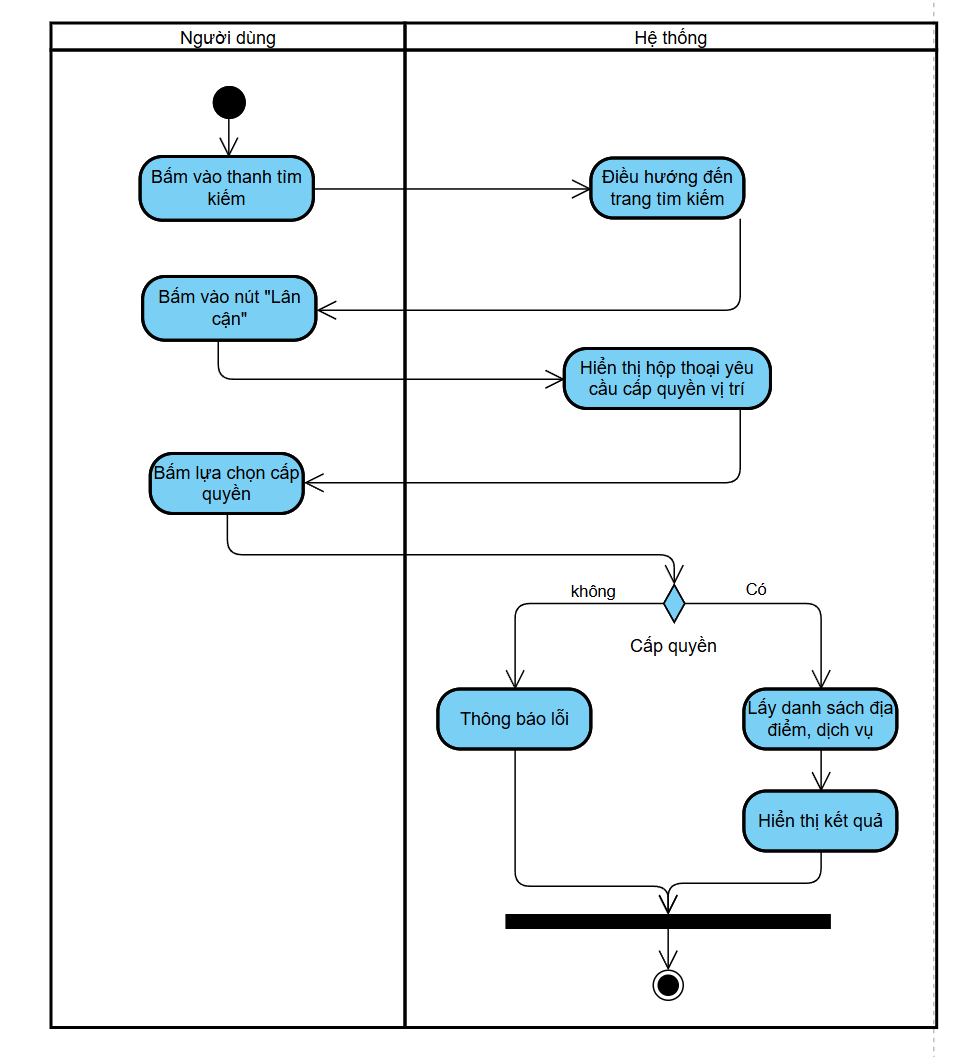
\includegraphics[width=0.5\linewidth]{figures/c3/3-3-7-ad.png} % Specified width
        &
        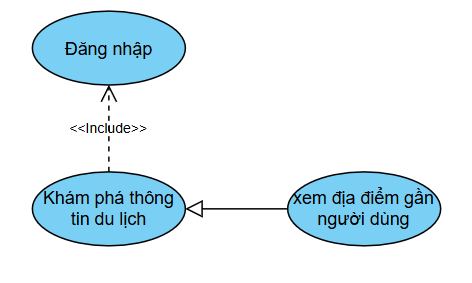
\includegraphics[width=0.45\linewidth]{figures/c3/3-3-7-rd.png} \\ % Specified width
        \hline
    \end{tabular}
\end{table}

\begin{figure}[H]
    \centering
    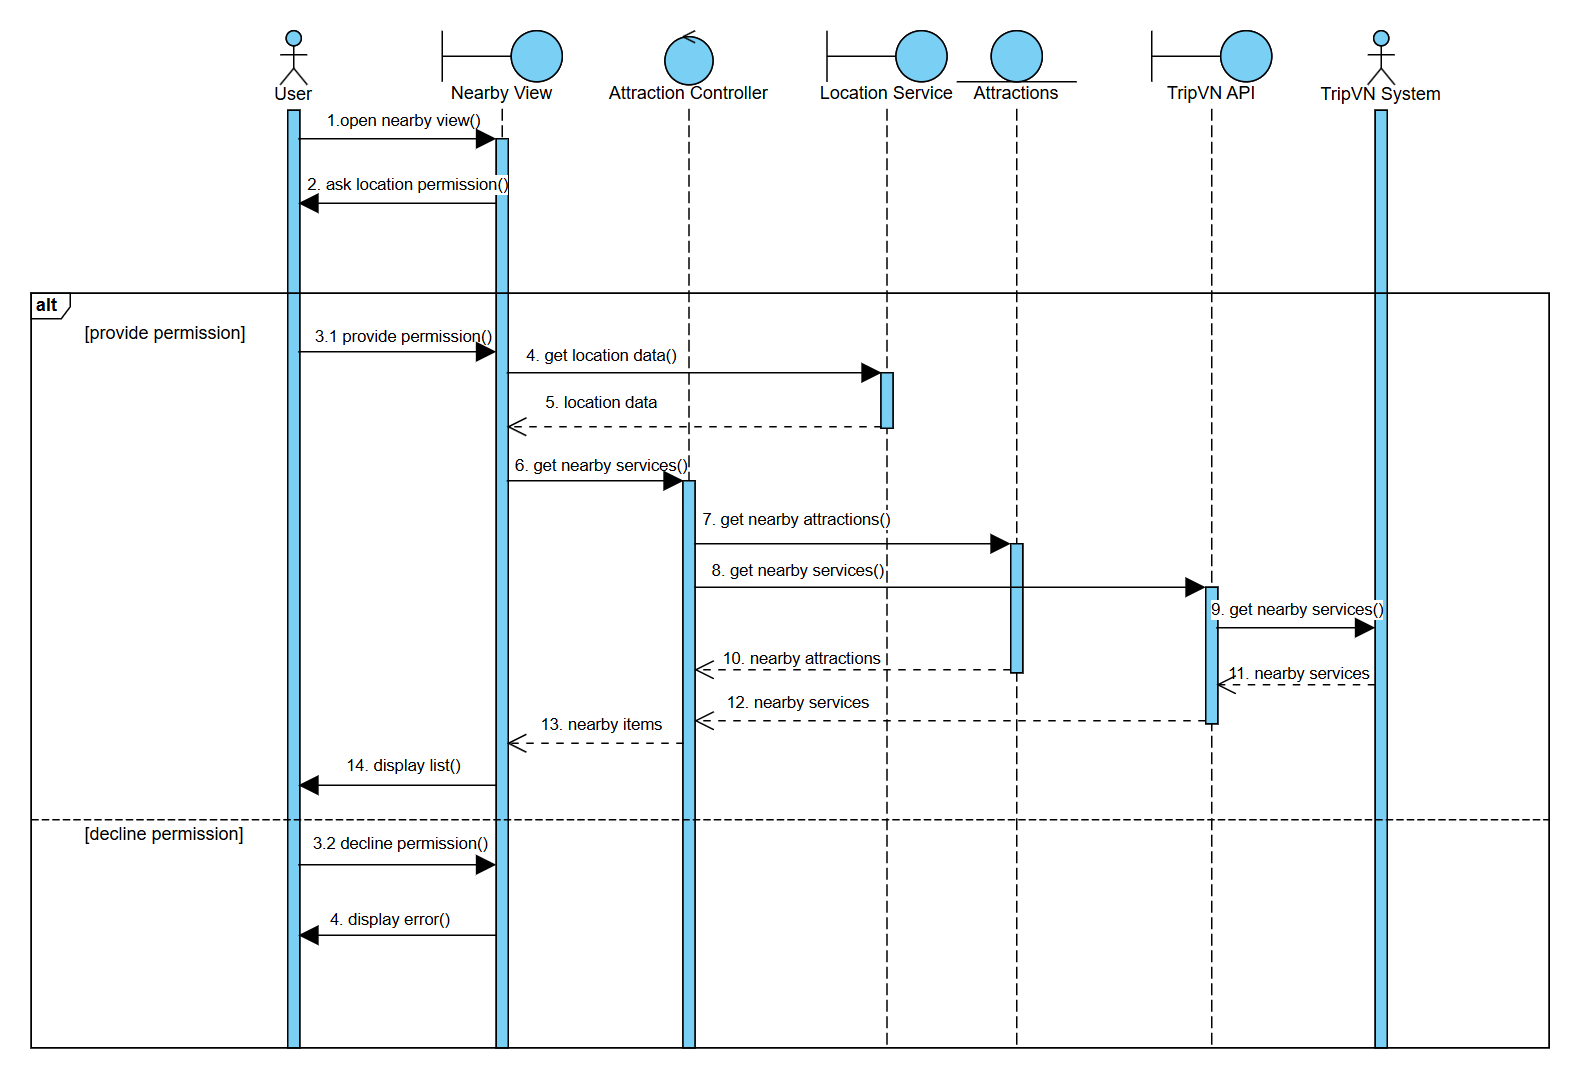
\includegraphics[width=1\textwidth]{figures/c3/3-3-7-sd.png} % Specified width
    \caption{Biểu đồ tuần tự ca sử dụng xem danh sách địa điểm gần người dùng.}
    \label{fig:3-3-7-sequence-diagram}
\end{figure}